\documentclass{article}

\usepackage{fancyhdr, ragged2e, indentfirst, longtable, tabu, graphicx, float, hhline, makecell, bookmark}
\usepackage[table]{xcolor}
\usepackage[letterpaper, total={7in, 9in}]{geometry}

\graphicspath{ {./imgs/} }

\makeatletter
\title{Documento de Arquitectura del Software} \let\Title\@title
\date{Septiembre 2018} \let\Date\@date
\author{Ricardo Münch} \let\Author\@author
\makeatother

\pagestyle{fancy}
\fancyhf{}
\rhead{Versión: 1.0 \\ \Date}
\lhead{eFuel \\ DAS \\ Identificador del documento}

\lfoot{Confidencial}
\cfoot{iKels Consulting \\ \Date}
\rfoot{Pag. \thepage}

\renewcommand{\headrulewidth}{1pt}
\renewcommand{\footrulewidth}{1pt}
\renewcommand{\contentsname}{Índice}

\newcommand\Tstrut{\rule{0pt}{2.6ex}}       % "top" strut
\newcommand\Bstrut{\rule[-0.9ex]{0pt}{0pt}} % "bottom" strut
\newcommand{\TBstrut}{\Tstrut\Bstrut}       % top&bottom struts

\renewcommand{\cellalign}{cl}
\renewcommand\cellgape{\gape[t]}

\begin{document}

    \newgeometry{textwidth=12cm,textheight=10cm}
    \begin{titlepage}
        \huge{\Title}
        \begin{flushright}
            \Large{eFuel \\ Versión: 1.0}
        \end{flushright}
    \end{titlepage}

    \restoregeometry

    \newpage
    \tableofcontents

    \newpage
    \begin{center}
        \begin{tabular}{ |c|c|c|c| }
            \hline
            \rowcolor{gray!30}
            Fecha & Versión & Descripción & Autores \\ [0.5ex]
            \hline\hline
            29/09/2018 & 1.0 & Documento de Arquitectura & Ricardo Münch \\
            \hline
        \end{tabular}
    \end{center}

    \newpage
    \section{Introducción}
    El objetivo principal de la arquitectura del software es aportar conceptos y un lenguaje común que ayuden a describir el software y permita la comunicación entre el cliente y los diseñadores.

    \subsection{Propósito}
    Este documento busca hacer una abstracción de lo que será el sistema a través de algunas vistas de la arquitectura del mismo. Se pretende definir algunos elementos estructurales que describen el sistema \emph{eFuel}.

    \subsection{Alcance}
    A continuación presentamos una abstracción de la estructura que debe tener el sistema. El documento contempla la vista lógica, la vista de datos y las características no funcionales que debe tener el sistema.

    \subsection{Referencias}
    No hace referencia a ningún otro documento.

    \subsection{Vista Global}
    Este documento comprende 6 secciones en las cuales se elaboran los distintos aspectos de la arquitectura de \emph{eFuel}, tanto a nivel de software como de hardware. En la sección \ref{reprArq} se introduce la representación arquitectónica del sistema. Luego, en la sección \ref{metasArq}, se enumeran los objetivos y restricciones que suscriben la arquitectura presentada. Seguidamente, se describen las distintas vistas que conforman la arquitectura de la sección \ref{vistaCasosDeUso} a la \ref{vistaDatos}, teniendo en la sección \ref{vistaCasosDeUso} la Vista de Casos de Uso. Finalmente, la sección \ref{tamDesemp}.


    \section{Representación Arquitectónica} \label{reprArq}
    La representación arquitectónica de \emph{eFuel} está basada en el modelo de 4+1 vistas de Philippe Kruchten. En el transcurso del documento se tratarán más a fondo los detalles de cada una.

    \section{Metas y Restricciones Arquitectónicas} \label{metasArq}

    \vskip 2cm
    \section{Vista de Casos de Uso} \label{vistaCasosDeUso}
    En esta vista se describirá el sistema desde el punto de vista de los casos de uso. El sistema tiene 2 actores principales:

    \begin{itemize}
        \item \emph{Admin}: Administrador de CPI. Es un usuario de Umbraco, lo que quiere decir que cuenta con las credenciales para poder ingresar al back-end de Umbraco y tiene los permisos necesarios para administrar las entidades y los grupos de CPI.
        \item \emph{Retailer}: Representa a una cadena. Solo tiene acceso a la información referente a las tiendas y productos que pertenecen a la cadena.
    \end{itemize}
    En el back office de Umbraco en la sección Member, se creó un grupo llamado \emph{cpi-user} en el que los miembros pertenientes al mismo, tienen las credenciales necesarias para acceder al sistema CPI.
    
\pagebreak
    \subsection{Resumen de Casos de Uso}
    \newcounter{magicrownumbers}
    \newcommand\rownumber{\stepcounter{magicrownumbers}\arabic{magicrownumbers}}
    \begin{center}
        \begin{longtable}{ | l | l | c | }
            \hline
            \rowcolor{blue!25}
            \multicolumn{1}{|c|}{ID del Caso de Uso} &
            \multicolumn{1}{|c|}{Caso de Uso} &
            \multicolumn{1}{|c|}{Actor} \\
            \hhline{===}
            \endhead

            \endfoot

           CU-\rownumber & Iniciar sesión (Umbraco) & Admin \\ \hline
           CU-\rownumber & Consultar lista miembros & Admin \\ \hline
           CU-\rownumber & Gestionar miembro (CRUD) & Admin \\ \hline
           CU-\rownumber & Consultar grupos & Admin \\ \hline
           CU-\rownumber & Gestionar grupo (CRUD) & Admin \\ \hline
           CU-\rownumber & Asignar miembro/s a grupo & Admin \\ \hline
           CU-\rownumber & Remover miembro/s de grupo (CRUD) & Admin \\ \hline
           CU-\rownumber & Cambiar permisos de miembro & Admin \\ \hline

           CU-\rownumber & Gestionar contenido & Admin \\ \hline
           CU-\rownumber & Consultar lista de cadenas & Admin \\ \hline
           CU-\rownumber & Gestionar cadena (CRUD) & Admin \\ \hline
           CU-\rownumber & Consultar lista de productos & Admin \\ \hline
           CU-\rownumber & Gestionar producto (CRUD) & Admin \\ \hline
           CU-\rownumber & Consultar lista de productos UPC & Admin \\ \hline
           CU-\rownumber & Gestionar producto UPC (CRUD) & Admin \\ \hline
           CU-\rownumber & Asignar producto/s a producto UPC & Admin \\ \hline
           CU-\rownumber & Remover producto/s de producto UPC & Admin \\ \hline
           CU-\rownumber & Consultar lista de precios & Admin \\ \hline
           CU-\rownumber & Consultar lista de tiendas & Admin \\ \hline
           CU-\rownumber & Gestionar tienda (CRUD) & Admin \\ \hline
           CU-\rownumber & Asignar tienda a cadena & Admin \\ \hline
           CU-\rownumber & Consultar lista de zonas & Admin \\ \hline
           CU-\rownumber & Gestionar zonas (CRUD) & Admin \\ \hline
	       CU-\rownumber & Consultar lista de catálogo generales & Admin \\ \hline
           CU-\rownumber & Gestionar catálogo (CRUD) & Admin \\ \hline
           CU-\rownumber & Asignar producto/s a catálogo & Admin \\ \hline
           CU-\rownumber & Remover producto/s de catálogo & Admin \\ \hline

           
           CU-\rownumber & Iniciar sesión (CPI) & Retailer \\ \hline
           CU-\rownumber & Consultar lista de productos & Retailer \\ \hline
           CU-\rownumber & Importar precios desde archivo excel & Retailer \\ \hline
           CU-\rownumber & Consultar reporte precio producto & Retailer \\ \hline
           CU-\rownumber & Exportar reporte precio producto & Retailer \\ \hline
           CU-\rownumber & Filtrar reporte precio producto por fecha & Retailer \\ \hline
           CU-\rownumber & Consultar reporte precio histórico de producto & Retailer \\ \hline
           CU-\rownumber & Filtrar reporte precio histórico por fechas & Retailer \\ \hline
           CU-\rownumber & Consultar reporte gráfico dispersión por catálogo & Retailer \\ \hline
           CU-\rownumber & Exportar reporte gráfico dispersión por catálogo & Retailer \\ \hline
           CU-\rownumber & Filtrar gráfico dispersión por catálogo & Retailer \\ \hline
           CU-\rownumber & Filtrar gráfico dispersión por fecha & Retailer \\ \hline
           CU-\rownumber & Consultar lista de catálogos personalizados & Retailer \\ \hline
           CU-\rownumber & Gestionar catálogo (CRUD) & Retailer \\ \hline
           CU-\rownumber & Asignar producto/s a catálogo & Retailer \\ \hline
           CU-\rownumber & Remover producto/s de catálogo & Retailer \\ \hline

        \end{longtable}
    \end{center}
\pagebreak
    \subsection{Diagrama de Casos de Uso}
    Se separaron los casos de uso en varios diagramas para facilitar la lectura.

    \begin{figure}[H]
        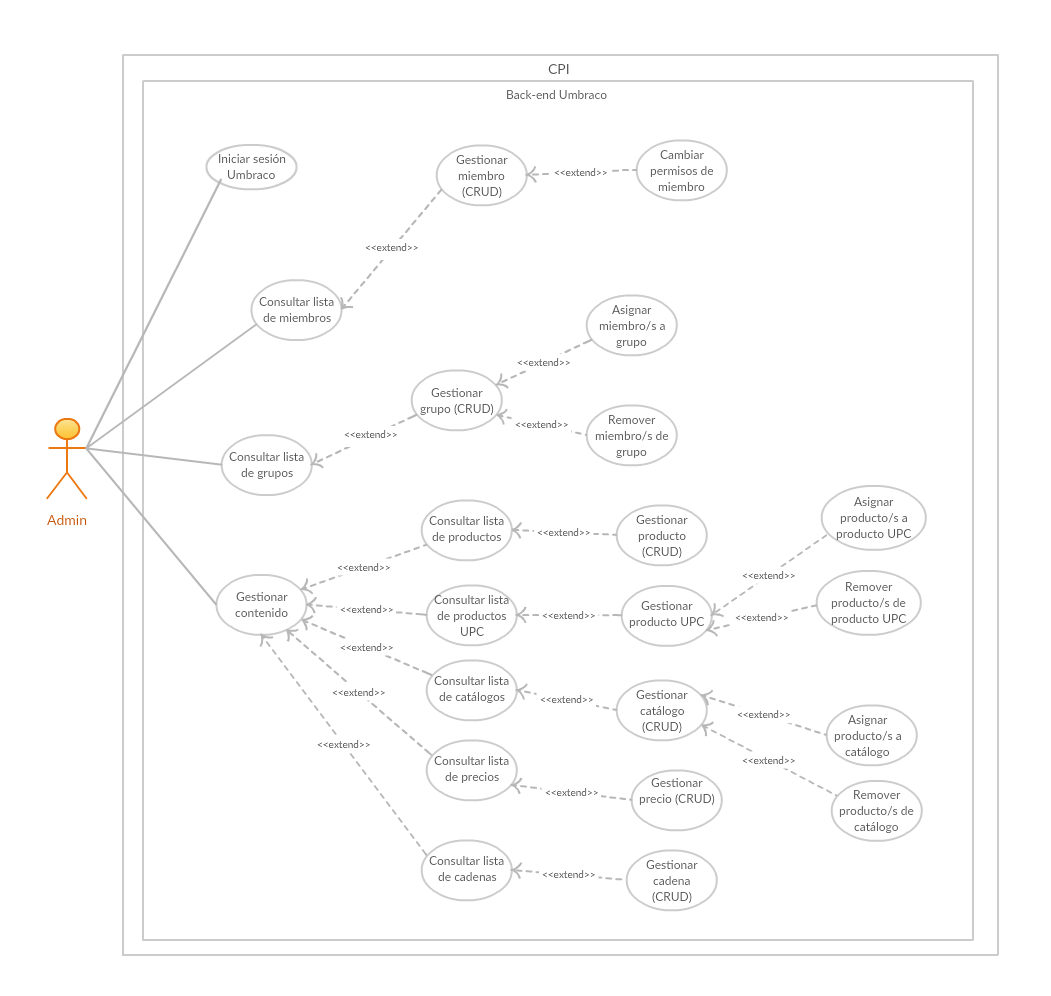
\includegraphics[width=\textwidth]{cu_admin.png}
        \caption{Casos de uso para usuario Admin}
        \label{fig:cu_admin}
        \centering
    \end{figure}

    \begin{figure}[H]
        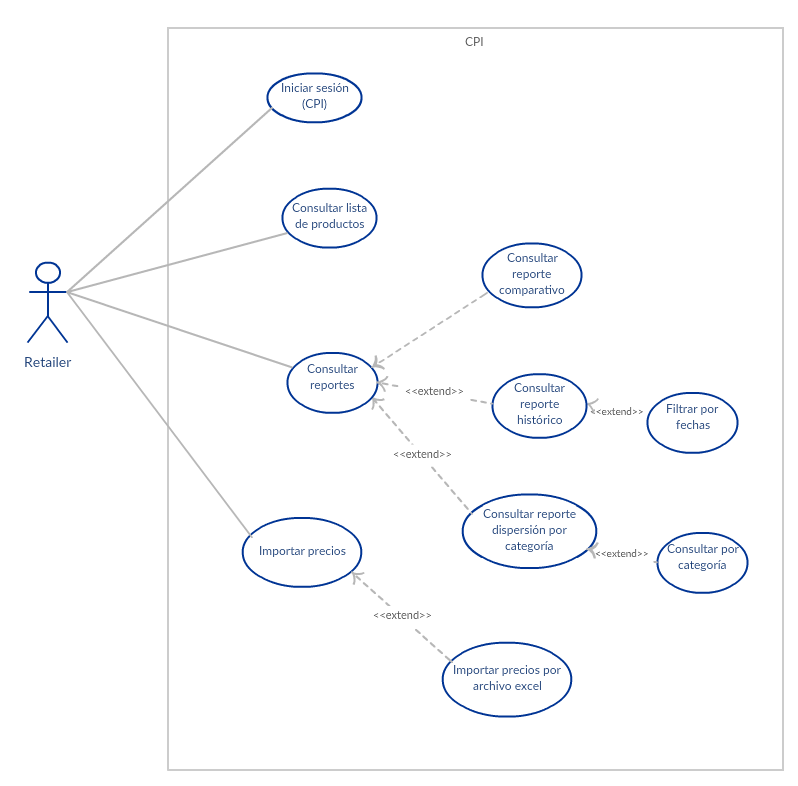
\includegraphics[scale=0.8]{cu_retailer.png}
        \caption{Casos de uso para usuario Retailer}
        \label{fig:cu_retailer}
        \centering
    \end{figure}
\pagebreak
    \subsection{Especificaciones de Casos de Uso}
    A continuación las narrativas de los casos de uso:

    \begin{center}
        \begin{longtabu} to 0.9\textwidth { | X[p] | X[p] | }
            \hline
            \multicolumn{2}{|l|}{
                \cellcolor{blue!25}{\large{\textbf{Caso de Uso:}} Iniciar sesión (Umbraco)}
            } \TBstrut \\
            \hline\hline

            \multicolumn{2}{|l|}{
                \makecell{\large{\textbf{Descripción:}} \\ El usuario quiere ingresar al back end de Umbraco.}
            } \\
            \hline

            \multicolumn{2}{|l|}{
                \makecell{\large{\textbf{Precondición:}} \\ Ingresar la dirección correcta del sitio en la barra de navegación.}
            } \\
            \hline


            \multicolumn{2}{|l|}{\cellcolor{blue!15}\large{\textbf{Flujo básico:}}}  \TBstrut\\
            \hline

            Actor & Sistema \TBstrut\\
            \hline
            1. El actor abre su navegador e introduce la dirección correspondiente al back end de Umbraco. &  \\ [0.3ex]
            \hline
             & 2. El servidor procesa la solicitud y envía al navegador del cliente una ventana para que el usuario se autentique. \\ [0.3ex]
             \hline
             3. El actor introduce su email y su contraseña. &  \\ [0.3ex]
             \hline
             & 4. El sistema valida la información del usuario y lo redirige al tablero (back end) de Umbraco. \\ [0.3ex]
             \hline\hline


            \multicolumn{2}{|l|}{\cellcolor{blue!15}\large{\textbf{Flujos alternos:}}}  \TBstrut\\
            \hline

            Actor & Sistema \TBstrut\\
            \hline
            1. El actor abre su navegador e introduce la dirección correspondiente al back end de Umbraco. &  \\ [0.3ex]
            \hline
             & 2. El servidor procesa la solicitud y envía al navegador del cliente una ventana para que el usuario se autentique. \\ [0.3ex]
             \hline
             3. El actor introduce su email y su contraseña. &  \\ [0.3ex]
             \hline
             & 4. El sistema no valida la información del usuario y lo redirige a la misma página de inicio de sesión indicándole que los datos introducidos son incorrectos. \\ [0.3ex]
             \hline\hline

            \multicolumn{2}{|l|}{
                \makecell{\large{\textbf{Poscondición:}} \\ El usuario se encuentra en el tablero de Umbraco.}
            } \\
            \hline
            \multicolumn{2}{|l|}{
                \makecell{\large{\textbf{Puntos de extensión:}} \\ No se requiere de otros casos de uso.}
            } \\
            \hline
        \end{longtabu}
    \end{center}
    \vspace{-4em}

    \begin{center}
        \begin{longtabu} to 0.9\textwidth { | X[p] | X[p] | }
            \hline
            \multicolumn{2}{|l|}{
                \cellcolor{blue!25}{\large{\textbf{Caso de Uso:}} Consultar lista de miembros}
            } \TBstrut \\
            \hline\hline
            \multicolumn{2}{|l|}{
                \makecell{\large{\textbf{Descripción:}} \\ El usuario quiere consultar la lista de miembros de CPI.}
            } \\
            \hline
            \multicolumn{2}{|l|}{
                \makecell{\large{\textbf{Precondición:}} \\ Haber ingresado al back end de Umbraco.}
            } \\
            \hline
            \multicolumn{2}{|l|}{\cellcolor{blue!15}\large{\textbf{Flujo básico:}}}  \TBstrut\\
            \hline

            Actor & Sistema \TBstrut\\
            \hline
            1. El usuario le da click a la sección "Members" en el tablero de Umbraco. &  \TBstrut\\
            \hline
            & 2. El sistema muestra el panel de miembros. \TBstrut\\
            \hline
            3. El usuario le da click a la carpeta "Members". &  \TBstrut\\
            \hline
            & 4. El sistema muestra la lista de los miembros de CPI. \TBstrut\\
            \hline\hline


            \multicolumn{2}{|l|}{\cellcolor{blue!15}\large{\textbf{Flujos alternos:}}}  \TBstrut\\
            \hline
            Actor & Sistema \TBstrut\\
            \hline
            1. El actor hace algo. &  \TBstrut\\
            \hline
             & 2. El sistema responde. \TBstrut\\
             \hline\hline


            \multicolumn{2}{|l|}{
                \makecell{\large{\textbf{Poscondición:}} \\ Aquí va la poscondición del caso de uso.}
            } \\
            \hline
            \multicolumn{2}{|l|}{
                \makecell{\large{\textbf{Puntos de extensión:}} \\ Aquí van los puntos de extensión del caso de uso.}
            } \\
            \hline
        \end{longtabu}
    \end{center}
    \vspace{-4em}


    \section{Vista Lógica} \label{vistaLogica}
    \subsection{Vista General}
    \subsubsection{Diagrama Conceptual (Modelo de Dominio)}
    \subsubsection{Diagrama de Clases}
    \section{Vista de Implantación} \label{vistaImplantacion}
    \subsection{Configuración Estándar}
    \subsection{Diagrama de Despliegue}
    \section{Vista de Implementación} \label{vistaImplementacion}
    \subsection{Vista General}
    \subsection{Diagrama de Componentes}
    \section{Vista de Datos} \label{vistaDatos}
    \subsection{Diagrama de Entidad Relación (ER)}
    \subsection{Diccionario de Datos}

    \section{Tamaño y Desempeño} \label{tamDesemp}

    \section{Calidad}
    \subsection{Mantenibilidad}
    \subsection{Flexibilidad}
    \subsection{Seguridad}
\end{document}

